\section{Priors}\label{sec:priors} 

In the previous section we calculated the likelihood of three candidate long-run frequencies. The examples presented in figure~\ref{fig:highlike_long-run_freqs} exhibit similar and high likelihood values, which suggests that the data could have well been generated from those three distributions of long-run frequencies. However, we observed that those distributions lead to different values of long-run mutual information (MI). This is a direct consequence of having limited samples; the more samples are available, the more the sample frequencies will converge to the long-run frequencies and thus the sample MI will converge to the long-run MI (see section ??). When the data is scarce, however, we can tackle the uncertainty in the inference of the long-run frequencies by making use of all relevant information about the system of study available at our disposal. In the context of computing mutual information, this translates into assigning weights to the candidate long-run frequencies the data could have been sampled from. Those weights will express our prior knowledge of the data and thus will depend on characteristics of the study: for example the employed recording technique, the brain area under study, the stimulus applied, the repertoire of possible neuronal responses, etc. Based on such weights we define the \textit{superdistribution} as the distribution of all candidate long-run frequencies. Note that this distribution lives in the space of candidate long-run frequencies. 
\mynote{Don't know if I should add an equation here to illustrate the superdistribution}

In order to illustrate what the superdistribution is, let us consider a discrete space of long-run frequencies that encompasses one, two or three spikes. We can conceptualize these distributions as lying on the surface of a triangle (see figure~\ref{fig:schematic_superdistribution}), where each dot illustrates one candidate long-run frequency, and the vertexes corresponds to firing \textit{only} one, two or three spikes. One possible superdistribution would be the one that favours the vertexes (figure~\ref{fig:schematic_superdistribution}B). This, however, is not a biologically realistic assumption as we know cells fire stochastically and do not always fire exactly the same number of spikes per bin. Based on the assumption that the cell under study has a low firing rate, and most likely only fires one or two spikes per bin, we could instead choose a superdistribution that assigns larger weights to those histograms (figure~\ref{fig:schematic_superdistribution}C). 



\begin{figure}
	\centering
	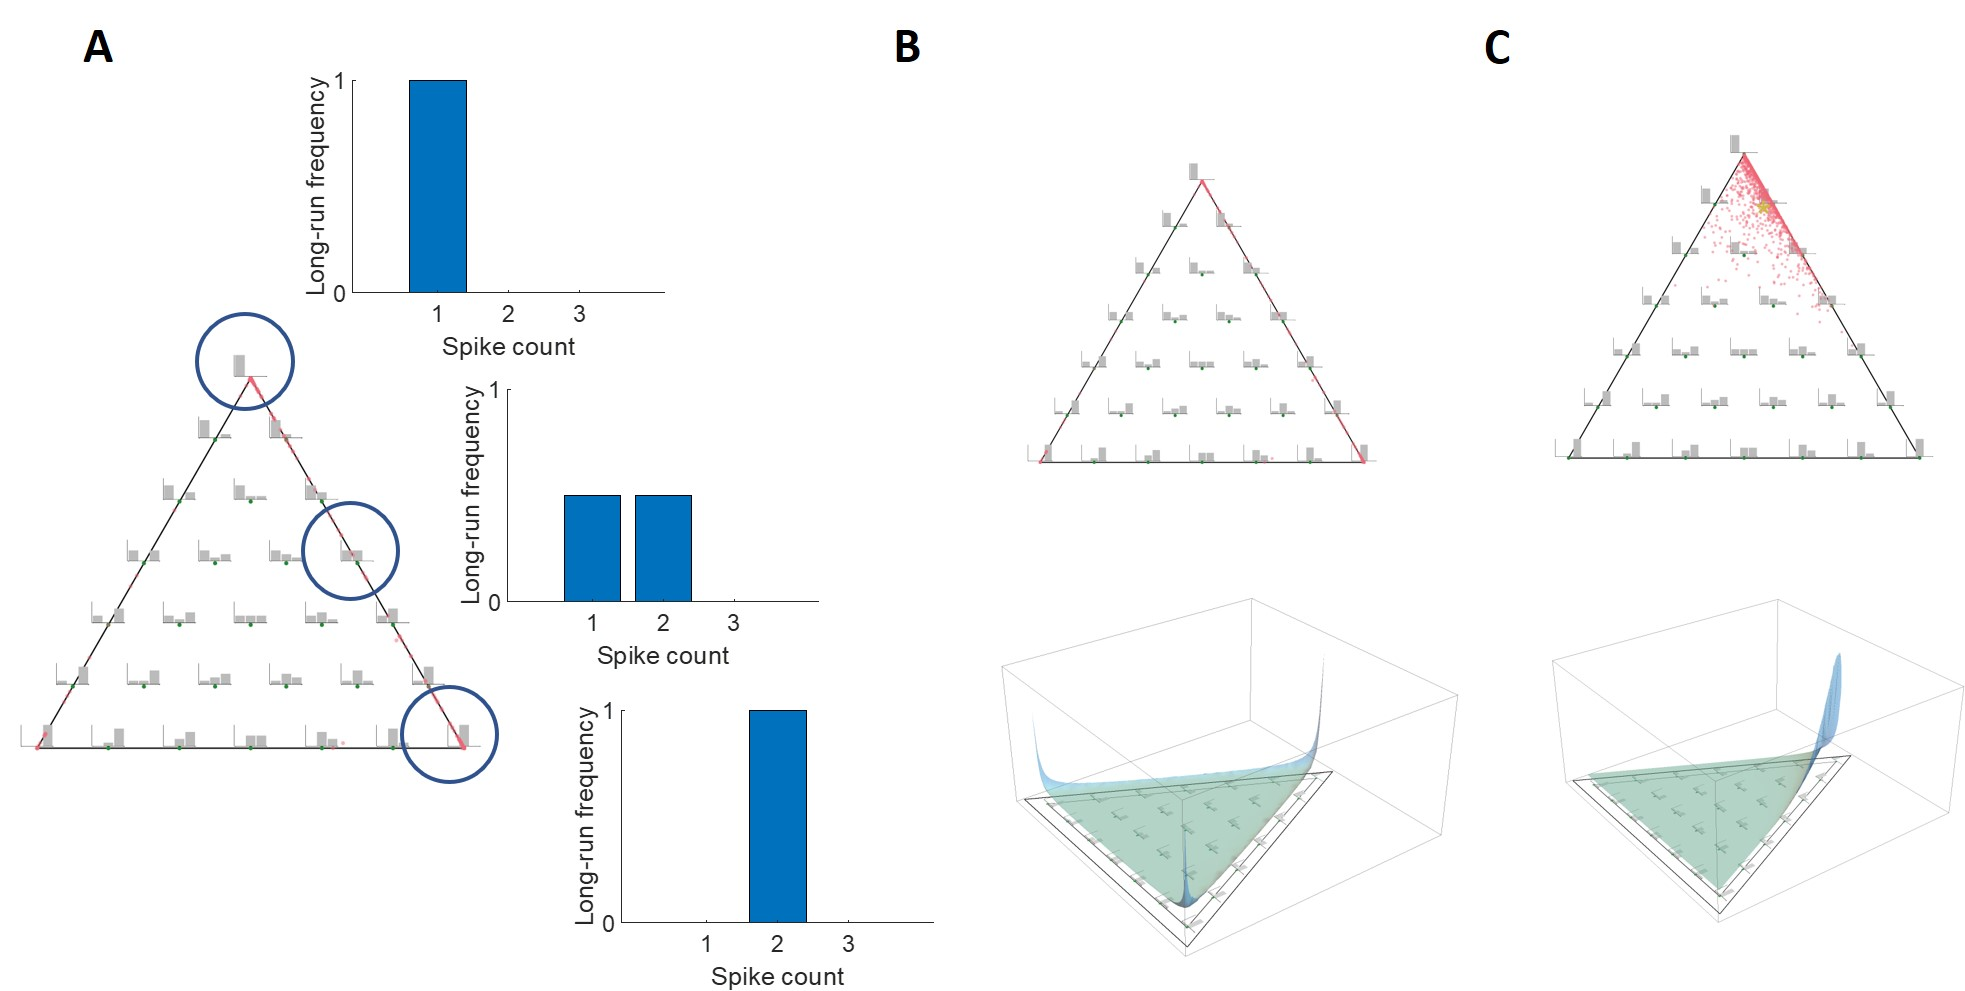
\includegraphics[scale=0.35]{superdistribution.jpg}%\\
	\label{fig:schematic_superdistribution}
	\caption{(DRAFT OF FIGURE) A: Schematic of the candidate long-run frequencies space. Each histogram corresponds to one candidate long-run frequency. B-C: Candidate long-run frequencies space (top) and superdistribution (bottom) for two different superdistributions. The red dots indicate the weights assigned to each long-run frequency. (check with Luca)}
\end{figure}


In the example of the NS cell figure ?? we presented three candidate long-run frequencies among all possible candidate distributions (figure~\ref{fig:highlike_long-run_freqs}). One possible superdistribution is the one that assigns the same weight to all candidate long-run frequencies, including the three examples. While this is a valid superdistribution (all superdistributions are) it is not biologically plausible, as it assigns equal weights to distributions that favour spiking at very high rates as well as non-spiking at all. Another possible superdistribution is the one that assigns weights different from zero to the distributions present in figure~\ref{fig:highlike_long-run_freqs}, and weights equal to zero to the rest. This could represent an improvement as the distributions with non-biologically plausible firing would get weights equal to zero. As for the three long-run frequencies shown in figure~\ref{fig:highlike_long-run_freqs}, we could assign their weights based on what we know a priori about this neuron. For example, this cell has a mean firing rate of 18.8 Hz, which favours histograms A C. If in addition we know that the cell tends to fire in bursts of two spikes, then the superdistribution should favour histogram A.  

Now let us turn to more general examples that illustrate superdistrubutions over a continuum of candidate long-run frequencies. From now on we will use the terms \textit{prior} and \textit{superdistribution} interchangeably. 

\begin{enumerate}[wide,label=(\roman*)] 
	
	\item {Uniform superdistribution over frequencies:} When there is no information available about the system under study the only choice left is to use an uninformative prior, which in a discrete case consists of a uniform distribution over all candidate long-run frequencies. However, in a continuous space, this doesn't hold anymore because this will depend on the parametrization of the space. We could, for example, choose a superdistribution that gives equal weights to equal intervals of conditional frequencies $f(r \|s)$. That is, the same weight to each hypercube $\prod_{r,s}\clcl{f(r\|s), f(r \|s) + \Delta}$, for fixed $\Delta$, for all values of $f(r \|s)$. Such a superdistribution is proportional to $\prod_{rs}\di f(r \|s)$.
		
	\item  {Uniform superdistribution over sequences:} Given some conditional frequencies $f(r \|s)$, a \textit{sequence} is defined as a set of n responses for each stimulus, with the responses appearing with frequencies $f(r \|s)$. Therefore, instead of using equal weights over the frequencies, we could use equal weights over the sequences. In this case the weights given to equal intervals in the frequency space will not be uniform, because some frequencies are realized by more sequences than others. Then we would obtain a superdistribution proportional to $\prod_{s} M\{f(r \|s)\}\,\di f(r \|s)$, where $M$ is a multinomial coefficient. \mynote{from Luca: will write the exact formula}
	
	\item {Non-uniform superdistribution over sequences:} Choosing a uniform prior over the sequences could be debatable from a biological point of
	view. If the responses for instance represent the firing rate of a population of cells, low responses should generally be expected more often than very high responses. Thus, more weight should be given to sequences in which low responses occur more frequently than high responses. This would
	lead to yet another superdistribution on the space of frequencies. \mynote{from Luca: will write the exact formula}
	
	\item {Not factorizable distribution over stimuli:} Should the superdistribution be factorizable over the frequency distributions? For example, for the two stimuli considered in the example above? Owing to biological constraints some similarity across the distributions should be expected. Thus such factorizability might be not be a sensible assumption.
	
\end{enumerate}

Different superdistributions reflect different assumptions about the data. But to which extent does the choice of superdistribution affect long-run MI? We explore this by comparing the values of long-run MI obtained with the four superdistributions listed above. We proceed as follows: From a given superdistribution we sample a pair of long-run response-frequency distributions. From this pair calculate the long-run mutual information. We then sample 20+20 responses from the pair, and calculate the sample mutual information obtained from such sample. We repeat this process ?? times. Figure~\ref{fig:superdistributions}  shows a scatter plot that tells us how often we should observe every pair of \[(\text{\small long-run mutual info},
\text{\small sample mutual info})\] under the assumption of the given superdistribution, for the four superdistributions described above. 

\begin{figure}[p]%{l}{0.5\linewidth} % with wrapfigure
	\centering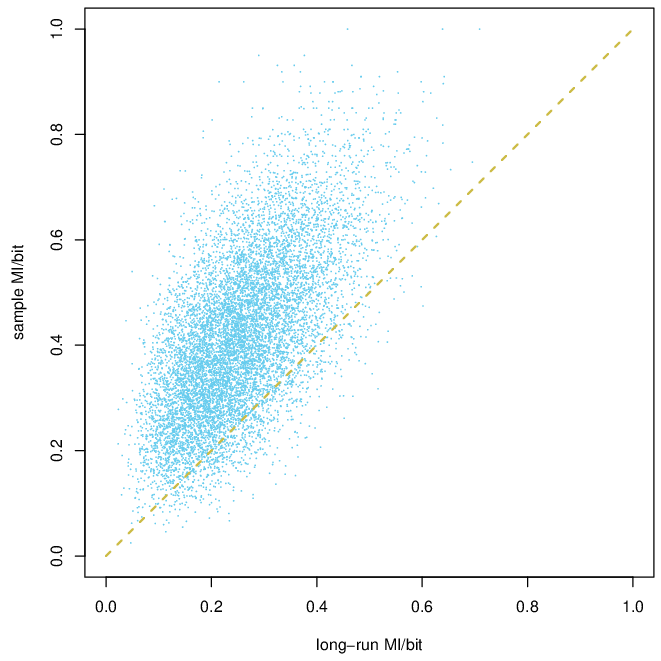
\includegraphics[width=0.49\linewidth]{scripts/scatter_unif10.png}%
	\hspace*{\stretch{1}}%  
	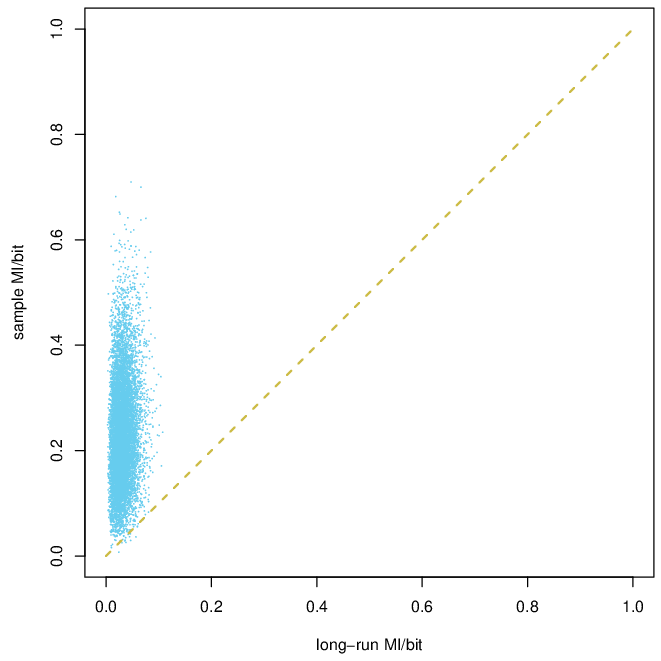
\includegraphics[width=0.49\linewidth]{scripts/scatter_peakcentre10.png}%
	\\[10\jot]%
	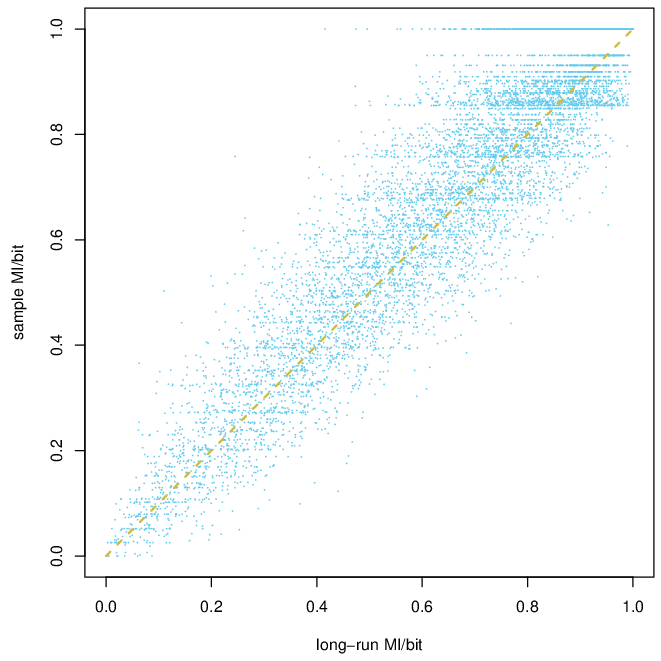
\includegraphics[width=0.49\linewidth]{scripts/scatter_biolunif.png}%
	\hspace*{\stretch{1}}%  
	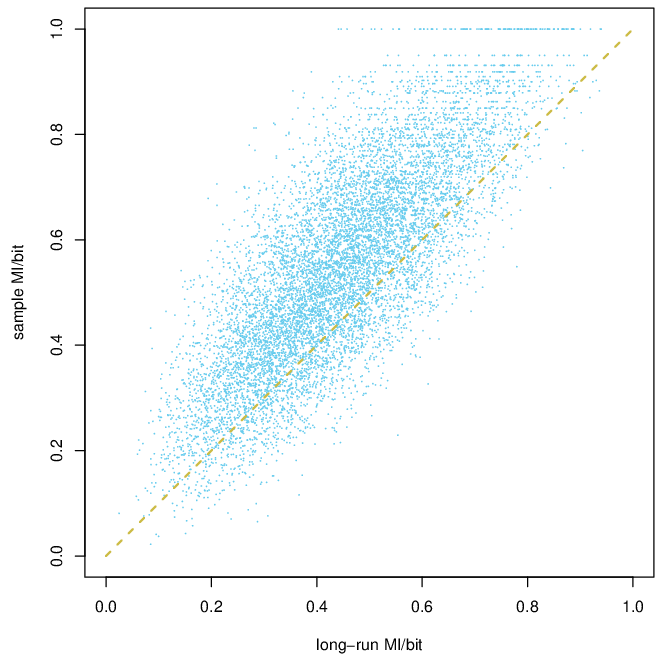
\includegraphics[width=0.49\linewidth]{scripts/scatter_Hunif_peak.png}%
	\\%
	\caption{Top left: uniform over frequencies. Top right: more uniform over
		sequences. Bottom left: low responses preferred. Bottom right: not
		factorizable over stimuli (positive correlation;
		hierarchic)}\label{fig:superdistributions}
\end{figure}% finite_sampling_bullshit.R


\mynote{Luca wrote this: Consequently, any
	inferences of long-run from sample and any quantifications of
	\enquote{bias} heavily depend on the assumed superdistribution. -- I would remove it from here and place it in the bias section}

The four examples of figure~\ref{fig:superdistributions} show that the joint distribution of long-run \amp\ sample mutual informations can be wildly different depending on the assumed superdistribution. Therefore, choosing a \enquote{default} superdistribution to be universally used for this kind of inference \citep[\cf][]{nemenmanetal2004} is not a sensible option, as any one-fits-all choice would simply fit every concrete case extremely poorly. At the same time, not choosing a superdistribution is impossible, as any proposed algorithm or formula to infer the long-run MI from the sample one is explicitly or implicitly choosing a superdistribution. Hiding such a choice will just lead to the same poor inferences as a default choice. We are then left with the need to choose a superdistribution as best as possible from considerations of the specific study. Any such choice, even if based on a very cursory analysis, will always be better than any default choice that completely disregards the specific case.

